\section{Simultaneous Left Inverse of Two Matrices}

We need \(H\in\mathbb{R}^{2\times 5}\) such that
\[
HG=I,\qquad H\tilde G=I
\]
An explicit matrix that works is
\[
H=
\begin{bmatrix}
-18/25&71/25&16/25&-2/5&0\\
8/25&-1/25&4/25&-3/5&0
\end{bmatrix}
\]
Direct multiplication gives
\[
HG=
\begin{bmatrix}
1&0\\
0&1
\end{bmatrix},
\qquad
H\tilde G=
\begin{bmatrix}
1&0\\
0&1
\end{bmatrix}
\]
Therefore this \(H\) recovers \(x\) from either measurement vector.


\begin{figure}[H]
    \centering
    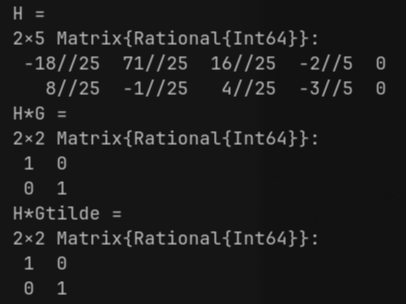
\includegraphics[width=0.4\textwidth]{img/2.png}
\end{figure}


\subsection{Code}
\begin{lstlisting}[language={}]
G = [2//1 3//1;
     1//1 0//1;
     0//1 4//1;
     1//1 1//1;
    -1//1 2//1]

Gtilde = [-3//1 -1//1;
          -1//1  0//1;
           2//1 -3//1;
          -1//1 -3//1;
           1//1  2//1]

H = [-18//25  71//25 16//25 -2//5 0//1;
       8//25  -1//25  4//25 -3//5 0//1]

H * G
H * Gtilde
\end{lstlisting}
